\documentclass{article}
\usepackage{graphicx,tikz}
\usepackage{fullpage}
\usepackage{amsthm}
\usepackage{amssymb}
\usepackage{amsmath}
\usepackage{algorithm}
\usepackage{algorithmicx}
\usepackage{algpseudocode}
\usepackage{booktabs}

\begin{document}
\title{\bf CS 273 Homework}
\author{Shiyu Ji}
\date{}
\maketitle

\section{Problem A}
Your task is to design a database for Amazon that sells books.
The following is the description of the application.
\begin{itemize}
\item Each book has a name and a publisher.
\item Each book has many versions. Each version has a version number, the year and date it was first published, and the authors.
\item Registered viewers can rate any version of a book. For each rate, we want to record its post date and rate.
\item For each registered viewer, we want to record his/her userID and password.
\end{itemize}
If you do not have sufficient information, please state your assumptions clearly.

(a) Draw an ER diagram for this application. Be sure to mark the multiplicity of each relationship of the diagram. Decide the key attributes and identify them on the diagram.

{\bf Answer}:
The ER diagram is given as follows.
\begin{quote}
\centering
\includegraphics[width=.8\textwidth]{er.eps}
\end{quote}

(b) Convert the above ER diagram into a relational schema. Merge relations where appropriate. Your solution should have as few relations as possible, but they do not need to be normalized. Specify the key of each relation in your schema.

{\bf Answer}: The relational schema is given as follows.
\begin{itemize}
\item Book(\underline{name, versionID}, publisher, year, date, authors)]
\item Rate(\underline{userID, versionID, bookName}, date, rate)
\item Viewer(\underline{userID}, password)
\end{itemize}

(c) Write a 3NF for the derived relational schema.

{\bf Answer}: A 3NF of the schema above is given as follows.
\begin{itemize}
\item Book(\underline{name}, publisher)
\item Version(\underline{versionID, bookName}, year, date, authors)
\item Rate(\underline{userID, versionID, bookName}, date, rate)
\item Viewer(\underline{userID}, password)
\end{itemize}

\section{Problem B}
The following questions refer to the database schema below: Product(pid, price, color), Order(cid, pid, quantity), Customer(cid, name, age).

(a) Write a query, in Relational Algebra, to return the names of customers who order at least one product with color ``Yellow''.

{\bf Answer}: $$\pi_{\texttt{name}} (\texttt{Customer} \bowtie \texttt{Order} \bowtie \sigma_{\texttt{color} = \texttt{Yellow}}(\texttt{Product})).$$

(b) Write a query in Tuple Relational Calculus and Domain Relational Calculus, to return the product with the highest price.

{\bf Answer}: 
\begin{itemize}
\item Tuple Relational Calculus:
$$\{t | t \in \texttt{Product} \wedge \forall s \in \texttt{Product} (s\texttt{[price]} \leq t\texttt{[price]})\}.$$
\item Domain Relational Calculus:
$$\{<i, p, c> | <i, p, c> \in \texttt{Product} \wedge \forall <i', p', c'> \in \texttt{Product} (p' \leq p)\}.$$
\end{itemize}

(c) Write an SQL query, to return the total quantity of products ordered by customers with age greater than 50.

{\bf Answer}:
\begin{verbatim}
select SUM(quantity)
from Order
where cid in (
    select cid
    from Customer
    where age > 50
);
\end{verbatim}

(d) Write an SQL query, to return the pid(s) of the most ordered product(s) (i.e. the product(s) with the highest total ordered quantities).

{\bf Answer}: 
\begin{verbatim}
select pid
from Product
where pid in (
  select pid
  from (
    select pid, SUM(quantity) as QuantitySum
    from Order
    group by pid
  )
  having SUM(quantity) in (
    select MAX(QuantitySum)
    from (
      select Sum(quantity) as QuantitySum
      from Order
      group by pid
    )
  )
);
\end{verbatim}

\section{Problem C}
We have an employee database with three tables. The Employee table stores information about employees. Every employee is identified by an {\bf EmployeeID}. The Department table stores information about each department. The Vacations table stores information about the total number of days each employee takes for vacation.
\begin{itemize}
\item Employee(\underline{EmployeeID}, FirstName, LastName, Office, Email, DepartmentID)
\item Department(\underline{DepartmentID}, DepartmentName)
\item Vacations(\underline{EmployeeID}, Days)
\end{itemize}

Answer the following queries using SQL and write its corresponding TRC if exists.

a) List the Office and Email of employee ``John Smith''.

{\bf Answer}: 
\begin{itemize}
\item SQL:
\begin{verbatim}
select Office, Email
from Employee
where FirstName = 'John' and LastName = 'Smith';
\end{verbatim}

\item TRC:
$$\begin{aligned}
\{t | &\exists s \in \texttt{Employee} (s\texttt{[Office]} = t\texttt{[Office]} \wedge s\texttt{[Email]} = s\texttt{[Email]} \\
&\wedge s\texttt{[FirstName]} = \texttt{'John'} \wedge s\texttt{[LastName]} = \texttt{'Smith'})\}.
\end{aligned}$$
\end{itemize}

b) List the number of vacation Days taken by each employee with the name ``John Smith''.

{\bf Answer}:
\begin{itemize}
\item SQL
\begin{verbatim}
select Days
from Vacations
where EmployeeID in (
  select EmployeeID
  from Employee
  where FirstName = 'John' and LastName = 'Smith'
);
\end{verbatim}

\item TRC:
$$\begin{aligned}
\{t | & \exists v \in \texttt{Vacations} (v\texttt{[Days]} = t\texttt{[Days]}
 \wedge \exists e \in \texttt{Employee} (e\texttt{[EmployeeID]} = v\texttt{[EmployeeID]} \\
&\wedge e\texttt{[FirstName]} = \texttt{'John'} \wedge e\texttt{[LastName]} = \texttt{'Smith'}))\}.
\end{aligned}$$
\end{itemize}


c) List the FirstName and LastName of all employees who never took a vacation day.

{\bf Answer}:
\begin{itemize}
\item SQL:
\begin{verbatim}
select FirstName, LastName
from Employee
where EmployeeID in (
  select EmployeeID
  from Vacations
  where Days = 0;
);
\end{verbatim}

\item TRC:
$$\begin{aligned}
\{t | & \exists s \in \texttt{Employee} (t\texttt{[FirstName]} = s\texttt{[FirstName]} \wedge t\texttt{[LastName]} = s\texttt{[LastName]}\\
& \wedge \exists v \in \texttt{Vacations} (v\texttt{[EmployeeID]} = s\texttt{[EmployeeID]} 
\wedge v\texttt{[Days]} = 0))\}.
\end{aligned}$$
\end{itemize}

d) List the DepartmentName of every department whose total number of vacation days taken by its employees is the largest among those of all the departments.

{\bf Answer}:
\begin{verbatim}
select DepartmentName
from Department
where DepartmentID in (
  select DepartmentID
  from (
    select DepartmentID, SUM(Days) as DaySum
    from Employee inner join Vacations
    on Employee.EmployeeID = Vacations.EmployeeID
    group by DepartmentID
  )
  having SUM(Days) in (
    select MAX(DaySum)
    from (
      select SUM(Days) as DaySum
      from Employee inner join Vacations
      on Employee.EmployeeID = Vacations.EmployeeID
      group by DepartmentID
    )
  )
);
\end{verbatim}

\section{Problem D}
We perform decomposition to normalize an original schema to be of certain normal forms. For such a decomposition to be ``equivalent'' to the original schema, it is desirable to be lossless. To study this concept, let us consider an original schema $R(A, B, C)$. Suppose we decompose $R$ into $R_1 (A, B)$ and $R_2 (B, C)$.

(a) Is this decomposition always lossless? Answer yes or no and briefly explain why.

{\bf Answer}: No. If there is a functional dependency $A \to BC$, then this dependency will be lost by such a decomposition. In particular, suppose two tuples have the same value of $B$ but different values of $A$ and $C$. Then the decomposed tuples in $R_1$ and $R_2$ give 4 possible combinations, implying it is impossible to recover the original schema.

(b) Give an example instance of $R$ (i.e. an example table with several tuples) and demonstrate its decomposition, to support your answer in (a).

{\bf Answer}: A ``lossy'' relation $R$ can given as follows:

\begin{tabular}{c c c}
$A$ & $B$ & $C$ \\
\hline
3 & 0 & 0 \\
4 & 0 & 1 \\
\end{tabular}

After decomposition $R_1$ contains $(3, 0)$ and $(4, 0)$, and $R_2$ contains $(0, 0)$ and $(0, 1)$.
Clearly the possible schema before the decomposition has another possibility: $(3, 0, 1)$ and $(4, 0, 0)$, implying it is impossible to recover the original schema.

\section{Problem E}
Given below is the set $\mathbf{F}$ of functional dependencies for the relational schema:
$$R = \{A, B, C, D, E, F\}$$
$$A \to BC$$
$$BD \to E$$
$$E \to F$$
$$F \to D$$
$$E \to D$$

1. Is the set $\mathbf{F}$ a minimal cover? Explain the reason. If $\mathbf{F}$ is not minimal cover, find a minimal cover for $\mathbf{F}$.

{\bf Answer}: No, $\mathbf{F}$ is not a minimal cover, since the dependency $E \to D$, which can be inferred by $E \to F$ and $F \to D$, is redundant.

By removing the redundant dependency we have the minimal cover as follows:
$$A \to BC$$
$$BD \to E$$
$$E \to F$$
$$F \to D$$

2. Based on the minimal cover for $\mathbf{F}$, produce a lossless BCNF decomposition for this schema. Is the result dependency-preserving? Explain why or why not.

{\bf Answer}: A lossless BCNF decomposition can be
$$R_1 (\underline{A}, B, C)$$
$$R_2 (\underline{E}, F)$$
$$R_3 (\underline{F}, D)$$
$$R_4 (\underline{A, E})$$
The BCNF above does not preserve the dependency $BD \to E$.

3. Based on the minimal cover for $\mathbf{F}$, produce a dependency preserving 3NF decomposition. Is the result redundancy free? Explain why or why not.

{\bf Answer}: A 3-NF decomposition can be
$$R_1 (\underline{A}, B, C)$$
$$R_2 (\underline{B, D}, E)$$
$$R_3 (\underline{E}, F)$$
$$R_4 (\underline{F}, D)$$
It contains redundancy of attribute $D$, which appears in both $R_2$ and $R_4$.

\section{Problem F}
1. Consider the relation Treatment and FDs below. Describe, with examples, two potential issues that can arise with this design.
\begin{itemize}
\item Treatment(doctorID, doctorName, patientID, diagnosis)
\item doctorID $\to$ doctorName
\item doctorID, patientID $\to$ diagnosis
\end{itemize}

{\bf Answer}: 
\begin{itemize}
\item A doctor may have many patients (e.g., 100 per month), then there are many repeated doctorName in the table, giving too much redundancy.
\item If one needs to update doctorName, it can easily give inconsistency to this table. If in the table of doctors, the doctorName is changed, then every doctorName in this table has to be updated as well. 
\end{itemize}

2. Prove that every two-attribute relation is in BCNF.
\begin{proof}
For any two-attribute relation $R(A, B)$, we have
\begin{itemize}
\item If without loss of generality $A$ is the primary key, then $A \to B$ is the only non-trivial dependency. 
\item If $A$ and $B$ together form the primary key, then every dependency is trivial.
\end{itemize}
For either case the condition of BCNF is satisfied.
\end{proof}

3. Prove that if relation $R$ is in 3NF and every key is simple (i.e., a single attribute), then $R$ is in BCNF.
\begin{proof}
Without loss of generality in any 3NF $R(A_0, \cdots, A_n)$ every non-trivial dependency $A_i \cdots A_j \to A_k$, we have two cases:
\begin{itemize}
\item $A_i \cdots A_j$ is a superkey, or
\item $A_k$ is in some key. Since every key in $R$ is simple, $A_k$ must be a key and thus a superkey.
\end{itemize}
Either case preserves the condition of BCNF.
\end{proof}

\section{Problem H}
There are two common methodologies (not specific techniques) to learn compact and meaningful word embeddings. List them and briefly describe the main idea.

{\bf Answer}:
\begin{itemize}
\item Dimensionality reduction on the word-word co-occurrence matrix. The main idea is to first find the global co-occurrence matrix and then store most of the important information in a fixed small number of dimensions, like a dense vector.
\item Directly learn low-dimensional word vectors. The main idea is instead of capturing global co-occurrence counts directly, we sequentially scan local windows and do prediction. We can incorporate a new sentence/document, or add a word to the vocabulary.
\end{itemize}

\section{Problem I}
(a) Given a query $q$ and a set of documents $d_1$, $d_2$, $\cdots$, $d_m$, use the vector space model to show how to rank documents. Assume $q$ and $d_i$ are sets of words.

{\bf Answer}:
In the vector space model, we represent each document and query as a vector in the space. Each term defines one dimension, and thus $n$ terms define a $n$-dimensional space. We rank the documents by their relevance with the query. We measure the relevance by the distance between the query vector and the document vector, e.g., the dot product between the vectors can be treated as the cosine similarity.

(b) Describe the intuition behind text length normalization and write down a normalization formula.

{\bf Answer}:
The intuition behind text length normalization is that the documents have different lengths, and many repeated occurrences in one document is much less informative than the first occurrence of the same word. Document length normalization is used to remove the chance that very long documents are more likely to be retrieved than the short ones, i.e., long documents usually have more terms and higher term frequencies, both of which may increase query-document similarity.

We can use the privoted normalization: let $|d_i|$ be the length of the document $d_i$. Then the normalization
$$PN_i : = 1- b + b\frac{|d_i|}{\sum_{j=1}^m |d_j|},$$
where $b$ ranges from 0 to 1. If the length $|d_i|$ is the old normalization of $d_i$, then $PN_i$ is the new normalization. 

(c) Describe the intuition behind language model smoothing and write down a smoothing function.

{\bf Answer}: 
In language model we treat each document as a sample drawn from a word distribution, and our goal is to learn the word distribution based on the given documents. A natural question is how to give the probability of a word which does not appear in the given document. If we assign some non-zero probability to these words, then the probabilities assigned to the words already in this document shall be discounted appropriately. This is basically the objective of the smoothing technique.

Simplified Jelinek-Mercer Smoothing:
$$p(w | d) := (1-\lambda) p_{ml}(w | d) + \lambda p(w | C),$$
where $p(w | C)$ is roughly TF-IDF of $w$ plus the length norm of $w$. $p_{ml}(w | d)$ is the frequency of $w$ in $d$. $\lambda$ is between 0 and 1.

\section{Problem J}
(a) Write down the objective function of $K$-means.

{\bf Answer}:
Suppose we use $K$-means to divide $n$ vectors $x_i$ into $K$ clusters. Then the objective function shall be
$$J := \sum_{j=1} ^K \sum_{C(i) = j} ||x_i - c_j||^2,$$
where $c_j$ is the average (centroid) of the cluster $j$. $C(i) = j$ denotes all the vectors $i$ that are grouped into cluster $j$. Our objective is to minimize $J$.

(b) Assume you have $n$ $d$-dimension vectors, write down the code of $K$-means to cluster these $n$ vectors to $K$ groups.

{\bf Answer}: Below is the pseudocode for $K$-means.
\begin{quote}
\centering
\begin{algorithmic}
\State Randomly partition the $n$ vectors into $K$ clusters: $C_1$, $\cdots$, $C_K$.
\State $flag \gets true$
\While {$flag$ is true}
  \State $flag \gets false$
  \For {each cluster $C_i$}
    \State Compute the average $c_i \gets \frac{1}{|C_i|}\sum_{k\in C_i} x_k$.
  \EndFor
  \For {each $x_i$}
    \State Set $c$ as the centroid of the cluster containing $x_i$
    \For {each $c_j$}
      \If {$|| x_i, c_j || < || x_i, c ||$}
        \State $c \gets c_j$
        \State $flag \gets true$
      \EndIf
    \EndFor
    \State  Set the cluster of vector $x_i$ as the one with centroid $c$
  \EndFor
\EndWhile
\end{algorithmic}
\end{quote}

(c) Explain three methods to measure the distance between two clusters for numerical data.

{\bf Answer}:
\begin{itemize}
\item Single link: smallest distance between an element in one cluster and an element in the other.
\item Complete link: largest distance between an element in one cluster and an element in the other.
\item Average: the averaged distance between an element in one cluster and an element in the other.
\item Centroid/Medoid: the distance between the centroids/medoids of the two clusters.
\end{itemize}

\section{Problem K}
Explain the connection and difference between two link-based ranking models: HITS and PageRank, and write down their formula.

{\bf Answer}:
Both the algorithms aim to find the authority webpages given the query. They both use the link model, i.e., hyperlinks can infer the notion of authority, and good authorities are often cited by many pages. Both the algorithms use iterative algorithms to reach the scores for ranking.

One of the major differences between HITS and PageRank is that HITS depends on the query, i.e., it needs to recompute all the scores per query, which could be computational expensive. Hence for efficiency HITS needs to know the small subset of relevant pages per query beforehand. Otherwise to deal with the entire webpages for each query is too expensive for web search. Also HITS maintains two scores (for hub and authority respectively) for each page, whereas PageRank has only one score. 

The equations used by the algorithms are given as follows.
\begin{itemize}
\item HITS:
$$a(p) := \sum_{i=1}^n h(i).$$
$$h(p) := \sum_{i=1}^n a(i).$$
Here we have $n$ pages. $a(i)$ denotes the authority score of page $i$, and $h(i)$ denotes the hub score of page $i$.

\item PageRank:
$$R(p) := c \sum_{q: q \to p} \frac{R(q)}{N_q},$$
where $N_q$ is the total number of out-links from page $q$. $c$ is a normalizing constant set so that the ranks of all pages sum to 1. $R(q)$ denotes the PageRank score of page $p$.
\end{itemize}

\section{Problem L}
In order to build a knowledge graph from a large text repository, we need to perform several tasks including entity extraction. Could you please describe these tasks and their connections?

{\bf Answer}:
The major tasks are given as follows:
\begin{itemize}
\item Entity Extraction. We use Named Entity Recognition to find and classify named entities in the unstructured text.
\item Triple Identification. Given the entities recognized by Entity Extraction, we try to find (subject, predicate, object) triples throughout the text. We first identify predicate phrases, and then find subjects and objects. Finally we evaluate the confidence score by using logistic regression classifier.
\item Entity Linkage. We associate an entity given by Entity Extraction to an entry in a knowledge base or expert system (e.g. Wikipedia). For each entity we may generate and rank candidates with the help of the knowledge base.
\item Predicate Linkage. Given the results from Triple Identification, we find synonymous predicates by using unsupervised method.
\end{itemize}

\section{Problem M}
Describe the basic steps of RandomForest.

{\bf Answer}:
In the training phase, we build $B$ decision trees as follows. To build each tree, we sample $n$ examples from the training dataset $X$, $Y$, and then use these sampled $n$ examples to train a decision tree.

In the classification phase we use the $B$ trees to predict and take the majority vote among them as the result.

\section{Problem N}
Explain how to cluster the following dataset. In a 2D plane, a group of points surround the other group of points.

{\bf Answer}:
We may use support vector machine with kernel method, i.e., to project these 2D points into some higher dimensional space and use linear SVM to do the classification, satisfying that the projection preserves the distance (or equivalents the dot product) between points. Clearly it is not appropriate linear SVM since in nature the dataset has VC dimension larger than 2.

\section{Problem O (Bonus Problem)}
Assume Facebook uses relational database technology to record its user information and user friendship information. It has two large tables (UserId, Gender), (UserId1, UserId2).

Denote the tables as
\begin{itemize}
\item User(\underline{UserId}, Gender)
\item Friend(\underline{UserId1, UserId2})
\end{itemize}

1. Writing a SQL query to list all of distinct 2-hop female friends of user ``Mary''.

{\bf Answer}:
\begin{verbatim}
select *
from User
where UserId in (
  select UserId2
  from Friend
  where UserId1 in (
	  select UserId2
    from Friend
    where UserId1 = 'Mary'
  )
)
\end{verbatim}

2. Writing a SQL query to find the user who has the maximal number of 2-hop friends.

{\bf Answer}:
\begin{verbatim}
select A.UserId1, COUNT(B.UserId2) as N
from Friend A, Friend B
where A.UserId2 = B.UserId1
group by A.UserId1
having N in (
  select MAX(N)
  from (
    select A.UserId1, COUNT(B.UserId2) as N
    from Friend A, Friend B
    where A.UserId2 = B.UserId1
    group by A.UserId1
  )
)
\end{verbatim}

3. Propose a query that could not be easily expressed by SQL. Please explain why.

{\bf Answer}:
Such a query can be to find the user who has the maximal number of $k$-hop friends, where $k$ is given in the query.

The reason of difficulty is that the number of tables to join depends on $k$, which is dynamic. It is impossible to fix the SQL code without the knowledge of $k$.

\end{document}